\documentclass[a4paper,10pt,twoside,openright]{report}
\addtolength{\oddsidemargin}{-.5in}
\addtolength{\evensidemargin}{-.5in}
\addtolength{\textwidth}{3cm}
\addtolength{\topmargin}{-.875in}
\addtolength{\textheight}{1.75in}
% \textwidth 16.59cm
% \textheight 21.94cm

\usepackage{amsmath}
\usepackage{lscape}
\usepackage{graphicx}
\usepackage[margin=0pt,font=small,labelfont=bf,labelsep=endash]{caption}
\usepackage{pdfpages}
\usepackage{amssymb}
\usepackage[position=t,singlelinecheck=off]{subcaption}
\usepackage{amsthm}
\usepackage{rotating}
\include{qcircuit} % Package used for typesetting quantum circuits. Included in directory
\usepackage{sectsty}
\usepackage[numbers,sort&compress]{natbib} % Natbib package, supports more fancy ways of citing
\usepackage{bm} %Allows for boldface of Greek characters in math mode.
\usepackage{placeins}
% \usepackage{layouts} %Used to print page-widths
\usepackage{tikz} %For drawing figures. Might make compilation slow.
\sectionfont{\sffamily\Large}
\subsectionfont{\sffamily}
\usepackage[Bjornstrup]{fncychap}
\ChTitleVar{\raggedleft\LARGE\sffamily\bfseries}
\ChNumVar{\fontsize{76}{80}\usefont{OT1}{phv}{m}{n}\selectfont}
%%%\setlength{\parindent}{0in}
\newcommand{\comment}[1]{} %Creates a command that does nothing in order to allow in-line comments

\setlength{\marginparwidth}{0pt}
\hfuzz=10pt %disables warnings for overfull hbox upto 10pt. Used for chapter headings
% \pdfsuppresswarningpagegroup=1 % Disables warnings for multiple pdfs with grouping on same page
\usepackage{fancyhdr}
\usepackage{hyperref} %Adds hyperlinks to references
\hypersetup{
    % bookmarks=false,         % show bookmarks bar?
    unicode=false,          % non-Latin characters in Acrobat’s bookmarks
    pdftoolbar=true,        % show Acrobat’s toolbar?
    pdfmenubar=true,        % show Acrobat’s menu?
    pdffitwindow=false,     % window fit to page when opened
    pdfstartview={FitH},    % fits the width of the page to the window
    pdftitle={Entanglement of Weakly-coupled Carbon-spins in Diamond},    % title
    pdfauthor={M.A. Rol},     % author
    pdfsubject={Quantum Computation},   % subject of the document
    pdfcreator={Adobe},   % creator of the document
    pdfproducer={M.A.Rol}, % producer of the document
    pdfkeywords={Entanglement} {Quantum computing} {Interference}{Parity Measurements}{Quantum Error Correction}, % list of keywords
    pdfnewwindow=true,      % links in new window
    colorlinks=true,       % false: boxed links; true: colored links
    linkcolor=darkgray,          % color of internal links
    citecolor=darkgray,        % color of links to bibliography
    filecolor=magenta,      % color of file links
    urlcolor=darkgray           % color of external links
}
\usepackage{enumerate}
\usepackage{cleveref} %Adds the cref command for clever referencing
% \usepackage{svg}

\begin{document}

\newenvironment{changemargin}[2]{%
\begin{list}{}{%
\setlength{\topsep}{0pt}%
\setlength{\leftmargin}{#1}%
\setlength{\rightmargin}{#2}%
\setlength{\listparindent}{\parindent}%
\setlength{\itemindent}{\parindent}%
\setlength{\parsep}{\parskip}%
}%
\item[]}{\end{list}}

% 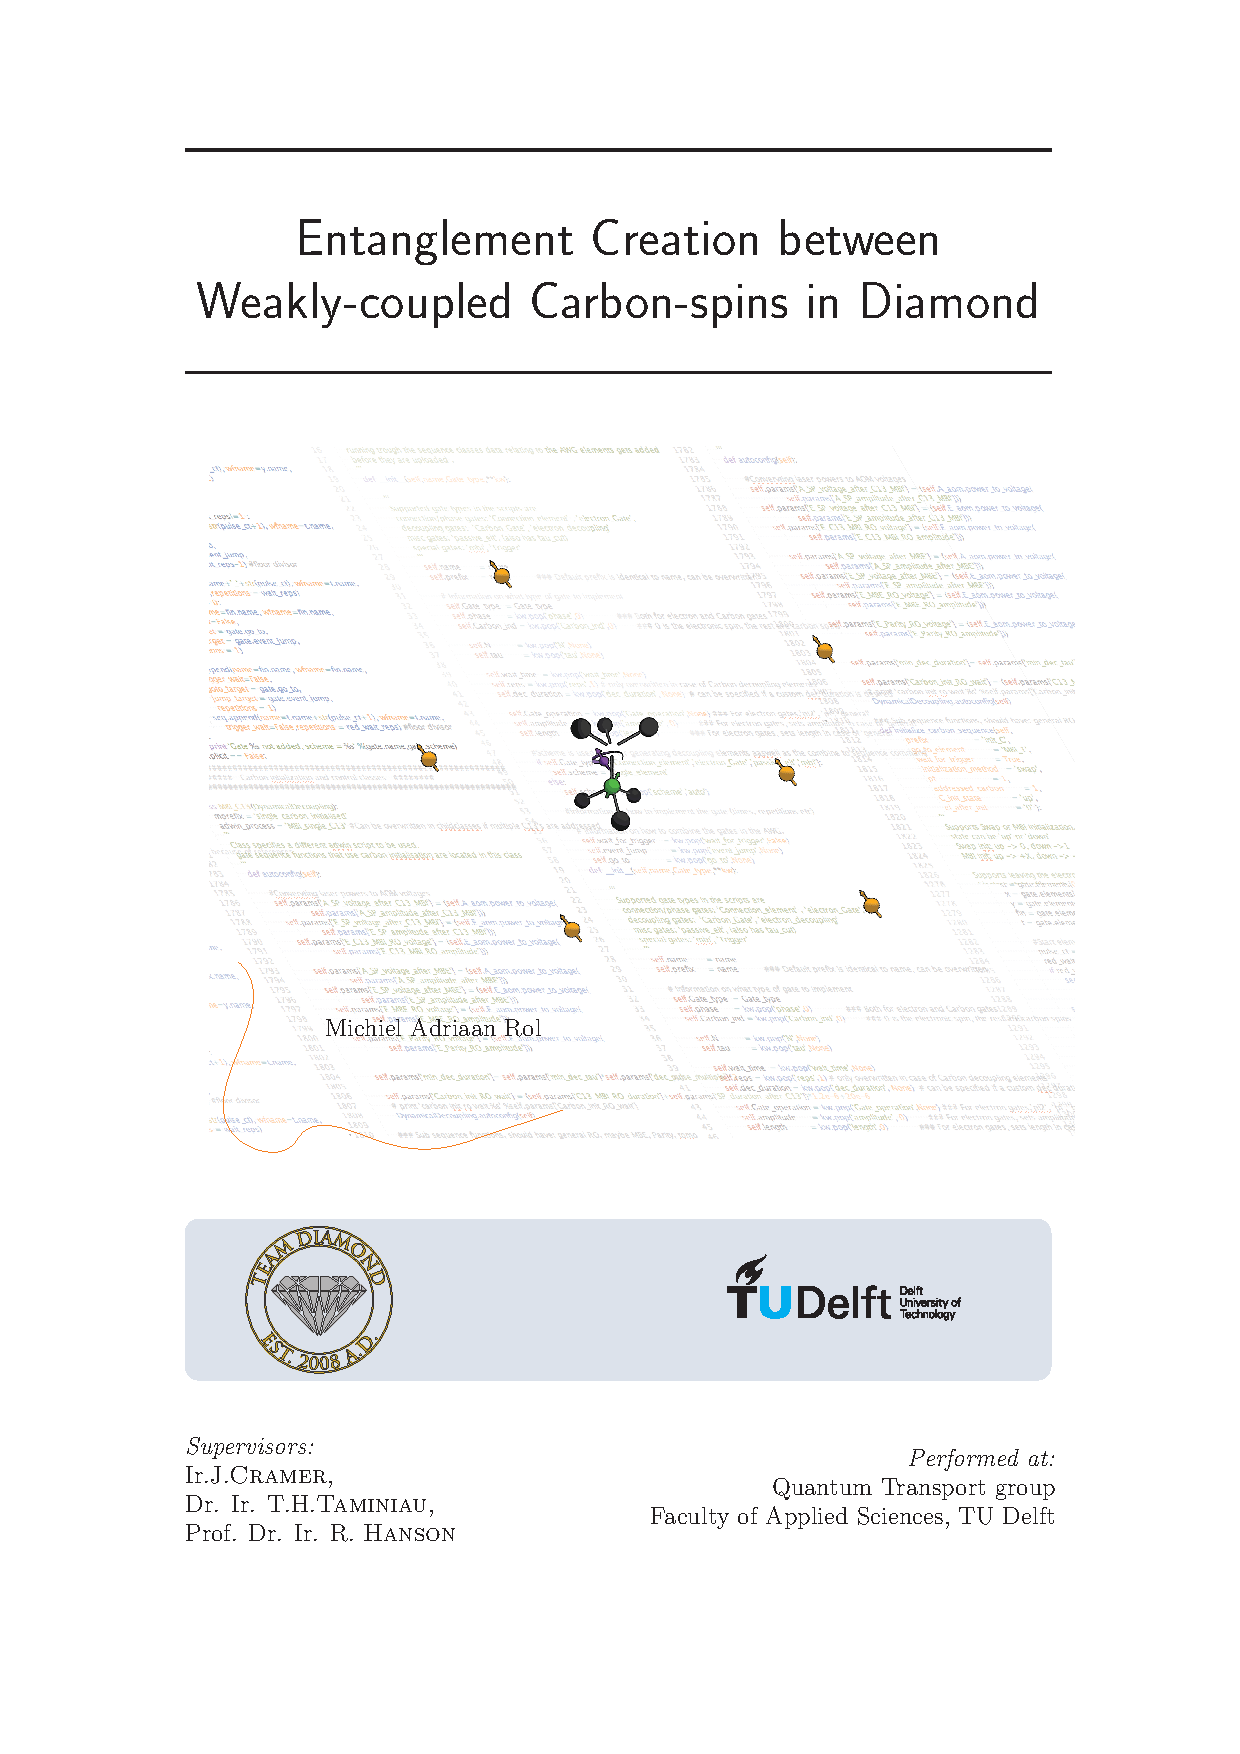
\includepdf{./Cover/cover_file.pdf}
% \newpage
% \thispagestyle{empty}
% \mbox{}
% \newpage

\begin{abstract}
Write Abstract here
\end{abstract}

\tableofcontents

\chapter{Introduction}
Although computers have increasingly become part of daily life they fall short when confronted with difficult problems  such as protein folding or searching a large unsorted database.
Quantum computers promise an exponential speedup for certain classes of problems making it possible to solve these problems on a human timescale.

A key challenge in building a large scale quantum computer is the presence of quantum errors.
To correct for these errors parity



% Qauntum computation is cool
% Hurdle Errors -> error correction
% System of choice NV center
% Goal of project

%weakly coupled carbons in NV- environment provide a naturally occuring spin register making it a promising candidate for QC
% For large scale larger and  deterministically available spin registers are desirable
% here we show deterministic generation of entanglement paving the way for measurement based QEC.
%  Simultations indicate that it is possible to control even more Carbon atoms extending the register and performing full QEC

% An essential feature for a scalable quantum computer is the ability to correct for quantum errors.
% The Nitrogen-Vacancy center in diamond is a promising candidate for a scalable quantum computer.
% In order to perform

% This chapter will explain why building a quantum computer is cool/important/essential/someotherbigword
% Explain why quantum error correction is essential in achieving this goal
% Requirements to perform quantum error correction
% Explain NV natural candidate
% Requirements 3-5 qubits + entanglement.
% This thesis will demonstrate how to address weakly coupled carbon spins and create entanglement between them.

% Paragraph: Quantum is cool because exponential scale up allowing previously unattainable problems

%The Nitrogen-Vacancy (NV) center in diamond is a promising candidate for a scalable quantum computer.
% An essential feature for building a scalable quantum computer is the ability to correct quantum errors.
% A basic form of Quantum Error Correction (QEC)  (cite references, either in NV or global)
% A logical next step is to perform QEC based on repeated parity measurements. (needs clarification).
% In order to perform measurement based QEC one needs to be able to initialize, control, read-out and entangle up-to 5 qubits.

\section{Quantum Computing}
The idea of using a quantum mechanical system to simulate physics was first explored by Feynman\cite{Feynman1982Simulating}.
Because the number of operations required to simulate a quantum system scales exponentially with the number of particles in the system it is not feasible to classically simulate such a system.
By manipulating a quantum mechanical system directly this scaling problem can be circumvented.

It was the idea of quantum simulation that led to the idea of exploiting quantum effects to perform computations.
Shor's algorithm \citep{Shor1994Algorithms} is a prime example of how the advantageous scaling of quantum systems can be exploited toe perform more efficient computations.

Shor's algorithm is an algorithm for prime factorization, where the best known classical algorithms for prime factorization scale exponentially Shor's algorithm scales polynomially.
Because of  the speedup provided by Shor's and other quantum algorithms it is possible to solve classes of problems that were previously unsolvable, such as the breaking of RSA encryption that relies on prime factorization being a computationally hard problem.
%Look up TJ Ladd et al. 2010 nature. On exponential speedup and entanglement as key resource. Can I link entanglement as resource to the propagation of errors?
% Proof of concept exists (+ examples of basic algorithms) but key challenge is scaling it up
Shor's algorithm has been shown to work on a small scale quantum computer \cite{Vandersypen2001Experimental}.
However to take full advantage of the efficient scaling behaviour of quantum computations a scalable quantum computer is required.

\section{Quantum Error Correction}
One of the main challenges in creating a scalable quantum computer is the effect of errors.
Because a quantum computer uses entanglement between multiple qubits as a resource an error an a single qubit can quickly propagate trough the system.
Using quantum error correction (QEC) it is possible to correct for such errors.
The threshold theorem states the final error probability of a quantum algorithm on a large register can be made arbitrarily small, if the probability of an error on a single qubit is below a certain threshold and QEC is applied \citep{Mermin1990Extreme}.
This makes quantum error correction a stepping stone on the way to realizing a scalable quantum computer \citep{Nielsen2010Quantum}.

Experiments demonstrating a form of QEC have been demonstrated in a range of systems.
Codes correcting for one type of quantum error have been implemented with nuclear magentic resonance \citep{Cory1998Experimental,Moussa2011Demonstration}, trapped ions \citep{Schindler2011Experimental}  and superconducting qubits \citep{Reed2012Realization}.
Recently two groups have implemented three qubit gate based QEC using the nitrogen-vacancy (NV) center in diamond \citep{Taminiau2014Universal,Waldherr2014Quantum}.

Although schemes exist to implement a scalable quantum computer using a purely gate based architecture most approaches rely on correcting for quantum errors by performing repeated parity measurements. An example of such an approach is surface coding \citep{Fowler2012Surface}.
For this reason the present work will focus on performing the parity measurements required for such error correcting schemes.

QEC is similar to classical error correction trough majority voting.
In classical majority voting a single bit is encoded onto a \emph{logical} bit consisting of multiple regular bits.
When an error on a bit has occurred the original bit can be recovered by measuring all the individual bits and determining the original state by majority voting.

In QEC the quantum bit (qubit) is encoded onto a logical qubit consisting of multiple regular qubits.
A consequence of classical majority voting is that it destroys a quantum state because it requires all bits to be measured.
By measuring the parity of two qubits the difference between two states can be determined without measuring the individual states.
If two states are parallel in the parity basis the parity measurement will return a positive result, if they are anti-parallel a negative result.
Performing a parity measurement on multiple qubits allows quantum errors, such as a bit-flip, a phase-flip or the combination of both, to be diagnosed.

\Cref{fig:gate_circuit_3_qubit_QEC} shows a circuit diagram for three qubit measurement based QEC.
The state $\ket{\psi}_\mathrm{C2}$ is encoded onto a logical qubit consisting of qubits C1, C2 and C3.
A parity measurement is performed on qubits C1 and C2, and on C2 and C3,  by reading out an ancilla qubit $e$.
From the result of the parity measurements it can be determined on which qubit an error occurred.
Based on this result the error can be corrected.
Because the logical qubit does not need to be decoded to correct for the error it is possible to repeat the error correcting part of the circuit, thereby improving the protection of the qubit.
The original qubit can be recovered by decoding the logical qubit.

\begin{figure}[htbp]
    \centering
    \mbox{
    \Qcircuit @C=1em @R=.7em {
        &&&& \control &\cw & \cw &\cw & \cw &\cw & \cw &\cw & \control \cw &\\
        \lstick{\ket{0}_e }        & \qw & \targ &\targ & \meter \cwx &  && \lstick{\ket{0}_e}     &\qw & \targ & \targ & \meter &  \cw \cwx  &\lstick{\ket{0}_e} &\qw&\qw &\qw &\rstick{\ket{0}_e} \\
        \lstick{\ket{0}_{\mathrm{C1}}}     &  \targ \qwx[1]& \ctrl{-1} &\qw & \qw &\qw&\qw& \qw &\qw & \qw &\qw & \qw & \multigate{2}{\mathrm{Corr.}} \cwx &\qw &\qw &  \targ \qwx[1] &\qw &\rstick{\ket{0}_{\mathrm{C1}}}\\
        \lstick{\ket{\psi}_{\mathrm{C2}}} &  \ctrl{1} & \qw &\ctrl{-2} & \qw &\qw&\qw&\qw  & \qw&\ctrl{-2} &\qw &\qw &\ghost{\mathrm{Corr.}}&\qw & \qw  &  \ctrl{1}&\qw &\rstick{\ket{\psi}_{\mathrm{C2}}}\\
        \lstick{\ket{0}_{\mathrm{C3}}}     & \targ   &\qw &\qw& \qw &\qw&\qw& \qw &\qw & \qw &\ctrl{-3} & \qw &\ghost{\mathrm{Corr.}}& \qw &\qw &  \targ&\qw &\rstick{\ket{0}_{\mathrm{C3}}}
        \gategroup{1}{3}{5}{13}{.7em}{--}  \
        % \gategroup{1}{3}{5}{12}{.7em}{_\}}
        % \gategroup{1}{13}{5}{13}{.7em}{_\}}
        % \gategroup{1}{1}{5}{2}{.7em}{_\}}
        % \gategroup{1}{14}{5}{14}{.7em}{_\}}
        }
    }
    \caption{Gate circuit for three qubit error correction. First the state of $C2$ is encoded onto three qubits.
    To diagnose an error an ancilla qubit is used to perform two parity measurements on the encoded qubits.
    The result of these measurements is used to determine what gates to apply to correct for the error if it occurred.
    These error correcting operations (in the dahsed lines) can be repeated to continuously protect the encoded qubits against quantum errors.
    The three qubit error correction code can correct for one type of quantum error. }
    \label{fig:gate_circuit_3_qubit_QEC}
\end{figure}

In order to implement measurement based error correction as depicted in \cref{fig:gate_circuit_3_qubit_QEC} we require initialization and control over three qubits and an ancilla that can be used to read out the main qubits.
Furthermore we need to be able to perform parity measurements on these qubits and deterministically perform operations based on the outcome of these parity measurements to correct for errors.

\section{The Nitrogen Vacancy Center in Diamond}
The NV-center is a promising candidate for quantum computation \citep{Childress2013Diamond}.
The NV-center is a naturally occurring impurity in diamond of which the electronic spin can be optically addressed and read out.
By applying microwave pulses to the NV-center it is possible to control and initialize strongly coupled spins in its environment \citep{Robledo2011HighFidelity}.
This spin register can be extended by addressing weakly coupled spins \citep{Taminiau2014Universal,Waldherr2014Quantum}.

Because of optical interface of the NV-center it is possible to link physically independent NV-centers together \citep{Bernien2013Heralded}. This has been used to demonstrate quantum teleportation \citep{Pfaff2014Unconditional}.

This unique combination of a local qubit register with an optical interface makes the NV-center a suitable system to implement a node based design for a scalable quantum computer\citep{Nickerson2013Topological}.

\section{Goal of the project}
In order to realize QEC at least three qubits are required to correct for a single type of error and more than five qubits are required to correct for a universal error.
Because the probability of finding enough strongly coupled carbons to implement QEC is small and goes down rapidly the more spins are required \citep{Waldherr2014Quantum,Taminiau2014Universal} we address weakly coupled spins using the methods developed by \citet{Taminiau2014Universal}.

The goal of this project is to implement  a parity measurement and demonstrate entanglement created by this parity measurement using weakly coupled spins in the environment of the NV-center.
The parity measurement is required for QEC in particular and measurement based approaches to quantum information in general.
This is done in a measurement environment that is designed from start to be compatible with the feed forward operations required for QEC.

The next chapter will explain the tools available to control the NV-center and strongly coupled spins.
\Cref{chap:addressing_weakly_coupled_carbons} will discuss how coherence can be extended
in order to control weakly coupled carbons.
In \cref{chap:control_weakly_carbon} these techniques are used to first initialize multiple weakly coupled carbon spins before creating entanglement using the parity measurement.
The last chapter will provide an outlook on how the capabilities developed can be extended to perform deterministic parity measurements and show simulations indicating that it is possible to perform multi qubit error correction using weakly coupled spins.

% Gives motivation for doing parity measurements based on the importance of QEC
% Clearly ending in several key requirements for the experiments:
        %  Control of enough qubits /carbons
        %  Feed forward -> Deterministic gates and dynamical operations
        %  Parity measurements
\chapter{Electronic spins in Diamond}
\label{controlingspinsindiamond}
%TODO_MAR:  Status: Up for revision
% TODO_MAR: Fix definition of weakly coupled carbons


% TODO_MAR: Rewrite introduction of diamond spin control chapter

%Explain here how general experiment looks

It has been shown that the nuclear- and electron- spin-state of the NV- center can be initialized, coherently controlled and read-out using microwave- and laser- pulses\citep{Robledo2011HighFidelity}. In these experiments two lasers that are resonant with transitions in the NV- center are used to initialize the electronic spin state. One of these two lasers is used to read out the electronic spin state and an off-resonant laser is used to reset the system. \comment{TODO_MAR: Check: Was the off-resonant laser already used in the Robledo paper?} Microwaves are used to drive transitions between the different nuclear and electronic spin states.

Strongly coupled nuclear spins can be initialized by conditionally rotating the electronic state to a state that is read out only if the Carbon is in the desired state, when the electronic state readout has a positive result the system is projected into the desired state. We call this Measurement Based Initialization (MBI).

Our experiments are build around the same basic tools\comment{As the Robledo experiment? }. Each experiment starts with a Charge-Resonance check \comment{Explain how CR-Check works? Ref?}that verifies if the lasers are still on resonance. After that the Nitrogen spin state is initialized using MBI.\comment{In what state is the Nitrogen initialized?} Once the system is initialized our actual experiment is performed. This consists of microwave pulses and a single or multiple readouts.

All experiments were performed on a custom-build cryostat setup operating at liquid helium temperatures described in detail in \citet[chap.~3]{Bernien2014Control}. The setup was additionally outfitted with a movable neodymium magnet that applied a magnetic field of ~300G to the sample.

\section{Spin Control}
\label{spincontrol}

The electronic ground state Hamiltonian can be written as\citep{Pfaff2013Quantum}: \comment{Do I cite wolfgang or Hannes or both?}
 \begin{equation}
H_{GS} = \Delta {S_z}^2 + \gamma_e \mathbf{B} \cdot \mathbf{S}
\end{equation}

With zero field splitting $\Delta \approx 2.88 \mathrm{GHz}$  and gyro-magnetic ratio $\gamma_e  = 2.802$ MHz/G . In this expression the interactions with the Nitrogen nucleus and the Carbon spin bath are not included. By applying a magnetic field $B_z$ a long the NV axis the degeneracy of the  $m_s =\pm1$ states is lifted by the Zeeman effect. A two level system that serves as a qubit can be defined with  $m_s=0:=|0\rangle$ and $m_s = +1 := |1\rangle$.

On the Bloch-sphere the state vector rotates around the quantization axis with a frequency depending on the energy splitting of the two states given by the Larmor frequency  $\omega_L =\Delta - \gamma_e {B_z} $.\footnote{When  $\omega_L$  is used as a vector it is pointing in the $\hat{z}$ direction.} By applying an external field a term is effectively added to the Hamiltonian, changing the quantization axis and thereby its evolution. By applying microwaves with the right frequency this can be used to selectively drive the transition from the  $|0\rangle$ state to the $|1\rangle$state\citet{Jelezko2004Observation}.


\section{Structure of a typical experiment}
% Explain pump laser and excitation laser,
% Explain experiment starts with checking if Lasers are on resonance
% Explain Nitrogen initialization to remove term from the Hamiltonian

% Explain structure of typical experiment and experimental setup
% Setup, same as in old papers. State temperature 4K, state that magnetic field is used.
%Structure.
%CR-check , Init electron with lasers, Init Nitrogen, do fancy pulse sequence, readout, possibly feed forward, more pulses, RO again.



% \section{Dynamical decoupling}
% DONT need to explain general dynamical decoupling?
%Explain what dynamical decoupling is, decoupling from environment by 'inverting' the enviroment thus reducing influence of decoherence causing carbons.
%Show figure from Tim's paper showing extended electron coherence times.
% Make bridge to next chapter by refering paper again showing that it's possible to control carbons in this way by resonantly doing this

% Chapter elaborates on general electronic spin control and the architecture of a typical experiment
\chapter{Controlling Weakly-coupled Carbon Spins}
The creation of entanglement is an essential capability for QEC in particular and quantum-computation in general.
This chapter demonstrates how weakly coupled nuclear spins can be initialized and read-out and how this can be used to generate entanglement between them.
The creation of entanglement is demonstrated with a quantum state tomography.

\section{Initialization and readout of single spins}
\label{sec:carbon_init_and_readout}
A weakly coupled spin can be initialized by conditionalizing on a readout result, similar to how nitrogen-MBI works.
A weakly coupled carbon spin can be read-out by using the $\pm \mathrm{x}$-gate to entangle the phase of the electronic-spin with the state of the nuclear spin and reading out the phase of the electronic spin.

%Explain Readout.
The gates used to initialize a weakly coupled nuclear spin are depicted in \cref{fig:gate_circuit_initialization}.
The circuit depicted in \cref{fig:gate_circuit_mbi_x-init} is used to perform a read-out along the $x$-axis.
By applying a $\pm y$-gate on the carbon before the initial $y$-pulse the state can be read out along the $z$-axis.

%Explain Initialization.
\begin{figure}[htbp]
    \centering
    \begin{subfigure}[t]{0.49\textwidth}
    \centering
    \caption{}
    \mbox{
        \Qcircuit @C=1em @R=.7em {
        \lstick{\ket{0}_e}                        & \gate{\mathrm{y}}  & \ctrl{1}       & \gate{\mathrm{x}} &\qw          &  \meter \\
        \lstick{\rho_\mathrm{m}}         & \qw              &  \gate{\pm \mathrm{x}}     & \qw    & \qw   & \qw}}
    \label{fig:gate_circuit_mbi_x-init}
    \end{subfigure}
    \begin{subfigure}[t]{0.49\textwidth}
        \centering
        \caption{}
        \mbox{
        \Qcircuit @C=1em @R=.7em {
            \lstick{\ket{0}_e} & \gate{\mathrm{y}}  & \ctrl{1} & \gate{\mathrm{x}} &\ctrl{1} &  \meter \\
            \lstick{\rho_\mathrm{m}}& \qw&  \gate{\pm \mathrm{x}}     & \qw    & \gate{\mp \mathrm{y}}    & \qw}}
        \label{fig:gate_circuit_mbi_swap-init}
    \end{subfigure}
    \caption{\Cref{fig:gate_circuit_mbi_x-init} MBI-based initialization into $\pm \ket{\mathrm{X}}$. Initializes the carbon into $\ket{X}_\mathrm{C} $ when $\ket{0}_e$ is measured and into $\ket{-X}_\mathrm{C} $ when $\ket{1}_e$ is measured for the electron.
    \Cref{fig:gate_circuit_mbi_swap-init} MBI-swap initialization into $ \ket{\mathrm{0}}$. Initializes the carbon into $\ket{0}_\mathrm{C} $ regardless of the electronic spin-state measured.}
    \label{fig:gate_circuit_initialization}
\end{figure}


% To initialize the nuclear spin
The initial pulse in \cref{fig:gate_circuit_mbi_x-init} brings the electronic spin in $\ket{X}_e$.
When the nuclear spin starts in the mixed state the system can be described by the tensor product of two density matrices:
\begin{equation}
    \rho_X \otimes \rho_m = \rho_X \otimes \rho_{X} +\rho_X \otimes \rho_{-X}
\end{equation}
By applying the $\pm{\mathrm{x}}$-gate  the electronic-spin picks up a phase depending on the nuclear spin-state:
\begin{equation}
     \rho_Y \otimes \rho_{X} +\rho_{-Y} \otimes \rho_{-X}
\end{equation}
By reading out the electronic spin along the $y$-axis the nuclear spin is projected into the $\ket{X}_C$ or $\ket{-X}_C$-state.
By conditionalizing on a positive readout result the state can be initialized into the $\ket{X}_C$-state.

By adding a second conditional gate (\cref{fig:gate_circuit_mbi_swap-init}) the nuclear spin is brought into the $\ket{0}_C$-state regardless of the measurement outcome for the electronic spin.

\paragraph{}
\Cref{fig:single_qubit_initialization} demonstrates initialization and readout.
In \cref{fig:carbon_init_x} carbon-1 is initialized into the $\ket{X}_C$-state and in \cref{fig:carbon_init_Z} it is initialized into the $\ket{0}_C$-state.
This is done by implementing the circuits depicted in \cref{fig:gate_circuit_initialization} and conditionalizing on a positive electron readout.

The carbon is read out using the same circuits.
The blue points correspond to $x$-readout, the green points to $y$-readout and the red-points to the $z$-readout.
The phase is sweeped to demonstrate that the readouts function as intended.
For a qubit in the $\ket{0}$-state the initial phase is undefined.

The combined fidelity of readout and initialization to the desired state is: $F(\ket{X}) = 90.57 \pm 0.85 \% $ for the $\ket{X}$-state and $F(\ket{Z}) = 93.00 \pm 0.31 \%$ for the $\ket{Z}$-state.
% Add description of features if still have time after finished today :)

\begin{figure}[htbp]
    \begin{subfigure}[t]{0.49\textwidth}\centering
        \caption{}
        \includegraphics{Img/RO_and_init_C1_X.pdf}
        \label{fig:carbon_init_x}
    \end{subfigure}
        \begin{subfigure}[t]{0.49\textwidth}\centering
        \caption{}
        \includegraphics{Img/RO_and_init_C1_Z.pdf}
        \label{fig:carbon_init_Z}
    \end{subfigure}
    \caption{Demonstration of carbon initialization and readout. In \cref{fig:carbon_init_x} carbon-1 is initialized in $\ket{X}$ and read-out. In \cref{fig:carbon_init_Z} carbon-1 is initialized in $\ket{0}$. Colored points correspond to readouts in different bases, blue to $x$-readout, green to $y$-readout and red to $z$-readout.}
    \label{fig:single_qubit_initialization}
\end{figure}


\section{The parity measurement}
Entanglement between two qubits can be created by performing a parity measurement on them and conditionalizing on the outcome.

A parity measurement does not measure the state of two qubits but measures if  two qubits are the same in a certain basis.
An example is the XX-parity measurement.
The XX-parity measurement returns a positive result if the the two qubits are the same in the $x$-basis and a negative result if the two are opposite.
That is it returns a positive result if the state is $\ket{X,X}$ or $\ket{-X,-X}$ and a negative result if the state is $\ket{X,-X}$ or $\ket{-X,X}$.
In general a two qubit parity operator has 2 eigenvalues, both are twofold degenerate.

The XX-parity measurement can be implemented on a weakly coupled carbon spins using the circuit depicted in \cref{fig:gate_circuit_general_Parity_RO}.
A parity measurement is very similar to the regular readout depicted in \cref{fig:gate_circuit_mbi_x-init}.
Once the electron is brought into a superposition the electron picks up phase when the $\mp \mathrm{x}$-gate is applied.
$+\pi/2$-phase when the carbon is in $\ket{+X}$ and $-\pi/2$-phase when the carbon is in $\ket{-X}$.
This is done for both carbons, when both carbons are in the same $x$-state the electron will pick up $\pi$-phase.
When they do not give the same result the phase cancels.
By reading out the electronic-spin along $x$ the parity is measured.
It should be noted that because we use a $\pm \mathrm{x}$-gate instead of a CNOT-gate an additional $\pi/2$-phase is added to the carbon states compared to a regular parity measurement.

\begin{figure}[htbp]
    \centering
\mbox{
\Qcircuit @C=1em @R=.7em {
\lstick{\ket{0}_e} &  \gate{\mathrm{y}}  & \ctrl{1} &  \ctrl{2} & \gate{\mathrm{y}}  &  \meter &\qw\\
\lstick{\ket{\psi}_{C1}} &  \qw & \gate{\pm \mathrm{x}}  &\qw   &  \qw   &\qw&\qw \\
\lstick{\ket{\psi}_{C2}}   & \qw   & \qw    & \gate{\pm \mathrm{x}}   &\qw & \qw &\qw}}
    \caption{Gate circuit for a XX-parity measurement. }
    \label{fig:gate_circuit_general_Parity_RO}
\end{figure}

\section{Quantum state tomography}
To demonstrate entanglement, entanglement must not only be created but it must also be verified that the entangled state is created.
This can be done by performing a quantum state tomography.
In a quantum state tomography the density matrix of a quantum state is reconstructed by repeatedly preparing the same state and gathering measurement statistics in different bases.

An arbitrary matrix can be described as a weighted sum of the Pauli-matrices and the Identity as in: \cref{eq:pauli}.
\begin{equation}
    \rho = I + \sum_{i,j} a_{i,j} \sigma_i \otimes \sigma_j
    \label{eq:pauli}
\end{equation}
By measuring the coefficients of \cref{eq:pauli}  the density matrix $\rho$ can be reconstructed completely.


\subsection{Readout}
To measure the coefficients of \cref{eq:pauli} single and multi qubit measurements are needed.
Single qubit measurements were described in \cref{sec:carbon_init_and_readout}.
The two qubit measurements required are very similar to parity measurements but do not need to preserve the state after the measurement.

The parity measurement depicted in \cref{fig:gate_circuit_general_Parity_RO} can be used to measure the XX-parity.
By changing the phase of one or two of the two $\pm \mathrm{x}$ gates Y-parities can be measured.
By applying a $\mp \mathrm{y}$ to one of the two carbons before the initial Y-pulse a Z-parity can be measured, care must be taken however that the phase difference between this gate and the $\pm \mathrm{x}$ on the corresponding carbon is $90^\circ$.

% How readout is implemented
\subsection{Initialization and tomography of multiple weakly coupled spins}
Before entanglement can be created the system must be initialized.
We verify that we have correctly initialized the qubits by performing a tomography.
The results are compared to the expected coefficients for the ideal case.

\Cref{fig:uu-init } shows a tomography of carbon-1 and carbon-4 initialized in the $\ket{00}$-state.
In the ideal case the single qubit Z-measurements and the ZZ parity are 1 and all other coefficients are 0.
The ideal case is represented by the gray bars in the \cref{fig:uu-init }.
The fidelity to the ideal case is $F = 81.43 \pm 1.68$ \%.

\Cref{fig:ud-init } shows a tomography of carbon-1 and carbon-4 initialized in the $\ket{01}$-state.
In the ideal case ZI =1 and IZ and ZZ are -1, all other coefficients are 0.
The ideal case is represented by the gray bars in the \cref{fig:ud-init }.
The fidelity to the ideal case prediction is $80.99 \pm 1.69$ \%.

\begin{figure}[htbp]
    \begin{subfigure}[t]{0.49\textwidth}\centering
        \caption{}
        \includegraphics{Img/uu-no-parity.pdf}
        \label{fig:uu-init }
    \end{subfigure}
    \begin{subfigure}[t]{0.49\textwidth}\centering
        \caption{}
        \includegraphics{Img/ud-no-parity.pdf}
        \label{fig:ud-init }
    \end{subfigure}
    \caption{ Quantum state tomographies of two initialized carbons. In \cref{fig:uu-init } the carbons are initialized into $\ket{00}$ with a fidelity of  $81.43 \pm 1.68$ \%.
    In \cref{fig:ud-init } the carbons are initialized into $\ket{10}$ with a fidelity of $80.99 \pm 1.69$ \%.
    }
    \label{fig:2qubitTomos}
\end{figure}

\section{Demonstrating entanglement between weakly coupled carbons}
Now that we are able to initialize multiple weakly coupled carbon spins and verify this with a tomography it is possible to demonstrate entanglement.
After the qubits are initialized an XX-parity is performed and the tomography is conditionalized on the negative readout result.

By conditionalizing on the negative readout result the carbons are projected into the negative-parity eigenstates of the XX-parity operator.
These are $\ket{-X,X}$ and $\ket{-X,X}$.
The tomography coefficient for the XX-parity is trivially -1.
The other coefficients depend on the initial state the parity was performed on.
The expected coefficients can be found as the expectation values of the operators on the state: $\bra{\Psi} \sigma_i \otimes \sigma_j \ket{\Psi}$ and are again depicted as gray bars.

\Cref{fig:uu-XX} shows the tomography for the negative XX parity of the $\ket{00}$-state.
$\ket{00}$ can be written in the X-basis as:
\begin{equation}
      \tfrac{1}{2} \left( \ket{X,X} + \ket{X,-X} +\ket{X,-X} + \ket{-X,-X} \right)
 \end{equation}
By measuring the negative XX-parity the state is projected onto:
\begin{equation}
    \tfrac{1}{\sqrt{2}} \left( \ket{X,-X} +\ket{X,-X} \right)
\end{equation}
The expectation for the ideal case is represented by the gray bars.
The fidelity to the ideal case prediction is $76.60 \pm 1.74$ \%.

\paragraph{ }
\Cref{fig:ud-XX} shows the tomography for the negative XX parity of the $\ket{01}$-state.
$\ket{01}$ can be written in the X-basis as:
\begin{equation}
    \tfrac{1}{2} \left( \ket{X,X} - \ket{X,-X} +\ket{X,-X} - \ket{-X,-X} \right)
 \end{equation}
By measuring the negative XX-parity the state is projected onto:
\begin{equation}
    \tfrac{1}{\sqrt{2}} \left( \ket{X,-X} -\ket{X,-X} \right)
\end{equation}
The expectation for the ideal case is represented by the gray bars.
The fidelity to the ideal case prediction is  $76.08 \pm 1.74$ \%


\begin{figure}[htbp]
    \begin{subfigure}[t]{0.49\textwidth}\centering
        \caption{}
        \includegraphics{Img/uu-XX-parity.pdf}
        \label{fig:uu-XX}
    \end{subfigure}
    \begin{subfigure}[t]{0.49\textwidth}\centering
        \caption{}
        \includegraphics{Img/ud-XX-parity.pdf}
        \label{fig:ud-XX}
    \end{subfigure}
    \caption{ Quantum state tomographies for entangled states created by measuring a negative XX parity.
    \Cref{fig:uu-XX} is the negative XX-parity of the state prepared in \cref{fig:uu-init }. It is in the $    \tfrac{1}{\sqrt{2}} \left( \ket{X,-X} +\ket{X,-X} \right)
$ with  $76.60 \pm 1.74\%$ fidelity.
    \Cref{fig:ud-XX} is the negative XX-parity of the state prepared in \cref{fig:ud-init }. It is in the $\tfrac{1}{\sqrt{2}} \left( \ket{X,-X} -\ket{X,-X} \right)$  with  $76.08 \pm 1.74$ \% fidelity.
    }
    \label{fig:2qubit_parity_Tomos}
\end{figure}

Some conclusion...


% Consists of several sub chapters
    %  theory of how weakly coupled carbons can be controlled
    %  Experiments used to characterize the environment and carbons
    %  Theory of initialization and readout of carbons
    %  Experiments showing single and multiple carbon initialization and readout
\chapter{Deterministic Parity Measurements}


\section{Entanglement}
%  Section gives definition of entanglement and refers to appendix for derivation of entanglement wittness.

\section{Verification of Entanglement}
% Section gives Results hopefully showing F>0.5 to Bell state with a cheer
%  Don't forget to elaborate where the error bars come from; statistical and does not include gate errors

%  Entanglement verification as test to check both feed forward and parity measurements
% Experiment (hopefully) showing F>0.5 to Bell state.
\chapter{Towards Quantum Error Correction}
Two more challenges remain to realize quantum error correction based on the parity measurements demonstrated in \cref{chap:control_weakly_carbon}.
First, to correct errors, gate operations that are conditional on the parity outcome are required.
Therefore the parity measurement must be accurate and preserve entangled state for both outcomes, unlike the probabilistic initialization and entanglement in this thesis.

Second, for error correction encoding in larger entangled states is required: at least three qubits for the simplest error correction and at least five qubits for correction of all types of errors.
In this chapter I address these two challenges and present simulations that indicate that multi-qubit parity measurements on weakly coupled spins are possible.

\section{Deterministic Parity Measurements}

An essential capability for QEC is the ability to perform different quantum operations based on a classical readout result.
An example of such an experiment is the deterministic creation of entanglement, as was demonstrated by \citet{Riste2013Deterministic} in a different system.

By applying an extra set of gates when the negative result is measured in a parity measurement the state can be transformed in the state that would have been created had the positive parity been measured.
This capability is particular important for QEC where the result of a parity measurement determines whether a correcting gate must be applied.

The main challenge when performing such operations is to keep track of the phase of the system while waiting for the readout result that determines which set of gates should be executed.
The measurement environment developed for the work in this thesis automatically keep track of phases and has been set up to be extendable and compatible with such feed forward capabilities.

%Several challenges -> extra phase, Keeping track of things
% An additional advantage of performing deterministic operations is that it can significantly speed up the rate at which experiments can be performed as it is no longer limited by part of the probabilistic initialization.


\section{Multi Qubit Control}
In order to implement QEC more than the two qubits that were addressed must be addressed.
To correct for a single type of quantum error 3 qubits are required.
To correct for any type of quantum error at least 5 qubits are required.


\subsection{Working of the simulations}
Simulations were performed to determine how many weakly coupled carbons can be controlled, on average, for an NV-center using dynamical decoupling.
In the simulations statistics were collected on 1000 NV-centers for a range of magnetic fields and three different carbon-13 concentrations.
%HOW MANY FOR EACH
For all NV-centers an environment of carbon-13 spins randomly placed on lattice points was generated.
For lower concentrations a larger environment was simulated such that the total number of simulated carbon spins was $\sim 300$ per NV-center for all concentrations.

NV-centers containing a carbon with a hyperfine coupling larger than $200\,\mathrm{kHz}$ were rejected as such spins are prone to decohere during the optical readout of the electron spin and their complex dynamics at moderate field complicate spin control of other spins (\cref{chap:addressing_weakly_coupled_carbons}).
In an experimental setting these carbons can be easily detected and the NV-centers rejected.

On the remaining centers the hyperfine coupling between each carbon and the NV-center as well as the resonance conditions of these carbons were calculated.
% 299 for \mu = 1.1%, 423 for 0.33% and even more for 0.011% (data loading crashes..).
At these resonances it was determined if a carbon can be selectively and coherently controlled.

%Definition addressable
As a figure of merit we take the fidelity $F$ of the electron spin after two consecutive $\pm \mathrm{x}$ gates.
The first gate entangles the electron spin with the nuclear spin and the second gate disentangles the two.
Reduced electron spin fidelity indicates gate imperfections or unwanted entanglement of the electron to the other carbon-13 spins.
The threshold for a carbon-13 to be considered controllable is set at $F = 90 \, \%$.

The fidelity is determined by sweeping the number of pulses at the resonance conditions and determining with what fidelity two consecutive $\pm \mathrm{x}$-gates can be implemented.
The accuracy with which the resonance can be addressed is limited by the resolution of the arbitrary waveform generator at $1\,\mathrm{ns}$.
The fidelity is determined under the assumption of perfect $\pi$ and $\pi/2$ pulses on the electron.

%Decoherence implemented
Additionally we require to be able to perform 10 such gates within the coherence time.
For simplicity we do not simulate the nuclear-nuclear interactions and instead set $T_2^*$ as in \cref{tbl:concentration_Tmaxes}.
% interpulse delay.
Finally, we set a maximum value for the inter pulse delay $\tau_{\mathrm{max}}$, to take into account the limited coherence for the electron at large $\tau$.
$\tau_{\mathrm{max}}$ is set at the values listed in \cref{tbl:concentration_Tmaxes}.
%Table listing times used
\begin{table}[htbp]
    \centering
    \caption{Coherence times and maximum resonance time as used in the simulations.}
    \begin{tabular}{ccc}
    Concentration &  $  T_{2,C}^* $ & $  \tau_{\mathrm{max} }$ \\ \hline
    $1.10\,\% $&  7ms & $10\,\mu\mathrm{s}$\\
    $0.33\,\% $&  45ms & $36.7\,\mu\mathrm{s}$\\
    $0.11\,\% $&  70ms & $100\,\mu\mathrm{s}$\\
    \end{tabular}
    \label{tbl:concentration_Tmaxes}
\end{table}

\subsection{Results of the simulation}
\Cref{fig:Simulations_avg_n_vs_bfield} shows the average number of addressable carbon spins as a function of magnetic field.
The number of addressable carbons increases quickly at first before a slow decay sets in.

The initial increase in the number of addressable carbons can be explained by the Larmor frequency becoming larger than the hyperfine interaction.
At low magnetic field ($\omega_L \sim A$) most spins undergo complex dynamics.
When the Larmor frequency becomes larger than the hyperfine coupling of a carbon spin it is in the simple regime where the resonances are narrow.
Because there is less overlap more spins can be addressed.
This increase drops off because eventually all spins are in the simple regime.

By increasing the magnetic field further the resonances both get narrower (\cref{eq:res_dip_width}) and move to shorter times \cref{eq:res_dip_loc}.
When the field becomes too high a resonance can become too narrow to accurately address.
This is limited by the 1ns timing resolution of the arbitrary waveform generator.
Therefore the number of addressable spins decreases at high fields.

For lower concentrations there are on average less spins undergoing complex dynamics for the same magnetic field.
This causes the initial increase in addressable carbons to be steeper at lower concentrations.

There is also a bias due to the rejection of carbons with $|A|>200\,\mathrm{kHz}$.
Not rejecting these carbons will lower the number of addressable carbons for low magnetic fields as the response of these carbons dominates the dynamical decoupling spectroscopy, while the number of addressable carbons will increase slightly in the high field limit were these carbons can be controlled trough dynamical decoupling.

\begin{figure}[htbp]
    \begin{subfigure}[t]{0.49\textwidth}\centering
        \caption{}
        \begin{tikzpicture}
            \node[anchor=south west,inner sep=0] at (0,0) {\includegraphics{Img/Simulations_avgN_vs_Bfield.pdf}};
            \node[font=\small, text = blue] at (5.0,4.90)  {$\mu = 1.10\,\%$};
            \node[font=\small, text = green] at (5.0,4.6)  {$\mu =0.33\,\%$};
            \node[font=\small, text = red] at (5.0,4.30)  {$\mu =0.11\,\%$};
        \end{tikzpicture}
        \label{fig:Simulations_avg_n_vs_bfield}
    \end{subfigure}
    \begin{subfigure}[t]{0.49\textwidth}\centering
    \caption{}
    \begin{tikzpicture}
        \node[anchor=south west,inner sep=0] at (0,0) {\includegraphics{Img/Simulations_Histogram_vs_Bfield.pdf}};
        \node[font=\small, text = black] at (5.4,4.90)  {$B = 700\,\mathrm{G}$};
        \node[font=\small, text = black] at (5.4,4.60)  {$\mu = 1.1\,\%$};
    \end{tikzpicture}
    \label{fig:simulations_histogram_vs_Bfield}
    \end{subfigure}
    \caption{Simulation results calculating the number of addressable carbons in NV-centers containing no carbons with hyperfine coupling larger than $200\mathrm{kHz}$. \subref{fig:Simulations_avg_n_vs_bfield} Average number of addressable carbons at different concentrations. \subref{fig:simulations_histogram_vs_Bfield} Normalized occurrences for $\mu = 1.1\,\%$ at $700\,\mathrm{G}$. The simulation indicates that an NV-center likely has 3 or more addressable carbons($P=89\,\%$), that there is a good chance that 5 or more carbons can be addressed ($P=57\,\%$) and that there is even a small probability of getting $\sim 10$ addressable carbon spins. }
    \label{fig:Simulation_results}
\end{figure}



% LONGER COHERENCE TIME
% When the concentration is lower the average separation between carbons and between carbons and the NV- centre is larger. This means that the coherence times are longer and that the coupling between a carbon and the NV- centre is on average weaker.

% OVERLAP
% One would expect that having less carbon atoms means less overlap in the resonances. Having less carbons might mean losing an easy to address carbon that is located close by. This effect is countered by also having some relatively weakly coupled carbons removed reducing overlap in resonances. The exact balance between these two effects depends on the configuration of each individual NV- centre.

% LONGER GATE TIMES
% Because the carbon atoms are coupled more weakly the magnetic field that is required before they can be resonantly addressed is much smaller. The downside of the weaker coupling is that the time it takes to implement a gate is much larger. Longer coherence times allow for longer gate times.

% LONGER RES TIME ALLOWED
% Because the longer coherence time a longer inter-pulse delay is allowed. This allows higher order peaks to be addressed at low magnetic fields. This allows additional carbon atoms to be controlled at low magnetic fields.

% DECLINE
% Eventually the dips become too narrow to address with the AWG. Because the width of the dips (\autoref{eq:res_dip_width}) depends on the strength of the coupling we expect this decline to set in earlier for lower concentrations as the carbons that are addressed are on average weaker coupled.


\paragraph{ }
\Cref{fig:simulations_histogram_vs_Bfield} shows the distribution of addressable carbons for a natural concentration of carbon-13 at the magnetic field that has the highest average number of addressable carbons.
It indicates that in most NV-centers ($89\,\%$) three or more carbons can be addressed and that in a reasonable fraction ($57\,\%$) of the samples five or more carbons can be addressed.
There are even rare occurrences where ten or more carbons can be addressed.

% % %%%%%%%%%
% Idem:

% Spins that have a stronger than average hyperfine-interaction show up outside or at the edge of the spin-bath collapse.
% Spins that are in the basic regime show up as a narrow dip.
% Going to larger $\tau$ separates these dips further as the order of the resonance $k$ increases.
% By looking at larger $\tau$ it is possible to resolve and address more resonances.
% Several spins in the basic regime have been identified 3 of these are visible as colored lines in \cref{fig:FP}.
% As computations are fundamentally limited by the coherence time there is a limit to the resonance-order that can be used to address carbons, making it impossible to resolve all weakly coupled spins.

% Besides the carbons in the basic regime there are also weakly-coupled carbons that are more strongly coupled.
% When a carbon in the complex regime is present in the NV-center this manifests itself as a resonance with strong oscillations on the side. Such a feature is also clearly visible in \cref{fig:FP}. We have identified the oscillations in the fingerprint as belong to a single spin which is denoted by the red line.

% When a weakly coupled carbon in the complex regime is present a significant part of the fingerprint spectrum is inaccessible for controlling other carbons making them an undesired feature when attempting to control weakly coupled carbon spins.



% Moved from identification section:
% \subsection{Effect of the magnetic field}

% Although increasing the magnetic field can improve the situation it is not always possible or desired.
% When the magnetic field becomes too strong too strong the resonances become narrower than the resolution of the Arbitrary Waveform Generator used to generate the pulses that address the resonances, making it impossible to address these resonances effectively.
% Simulations were performed (see \cref{chap:addressable_carbon_sims}) that indicate that for a natural carbon-13 concentration there is a range between 400G and 1400G where the magnetic field is optimal for controlling weakly coupled spins.

% Besides the spin environment there are other factors affecting the choice for magnetic field.
% Because the optical transitions used for readout and initialization depend on strain and magnetic field field\citep{Hensen2011MeasurementBased}, care must be taken when measuring that states do not mix in the excited state.
% This combined with the fact that few experiments have been performed at high magnetic field and low temperature make it more practical to settle for a more moderate magnetic field of 300G.

%  Outlook what more is needed for QEC
%  Short term outlook that indicates usefull 3 qubit QEC circuits
% Simulations showing long term outlook for quantum nodes


%%% FINAL stuff
% \input{references.tex}

%%% appendices
\appendix
%Appendix that explicitly calculates what states you get and how the gates work
\chapter{State Initialization}

%Derivation of the operation the gate circuit does and how it initializes

% Same for the Tomography/Readout

% Appendix that calculates what the tomography results will be for the different Bell states
\chapter{Bell State Tomography}
Derivation, what would a tomography of the Psi+ state look like?

% Appendix that performs derivation of entanglement wittness
\chapter{Entanglement wittness}
% Derivation of F>0.5 to Bell state as entanglement wittness

%Appendix showing how the simulations work and some more details about it.
\chapter{Simulations and Calculations for Number of Addressable Carbons}
\label{chap:addressable_carbon_sims}

\section{Scaling of number of resonances with magnetic field}
Starting from \cref{eq:res_dip_loc}

\begin{equation}
    \tau = \frac{(2k+1)\pi}{2\omega_L+A_\parallel}
\end{equation}
In the limit where $\bm{\omega_L} \gg \bm{A}$ the number of resonances $K$ of a single carbon between $\tau = 0$ and $\tau = T_{\mathrm{DD},e}$ scales linear with the magnetic field: $N_k \propto \omega_L$.

At the same time the width of these resonances decreases quadratically with magnetic field (\cref{eq:res_dip_width}).
\begin{equation}
    \Delta = \frac{A_\perp }{2\omega_L^2}
\end{equation}
Combining these two we find that the number of resonances $N$ that fit between two orders to increase linearly with magnetic field.
\begin{align}
N_k -N_{k-1} = \frac{\tau_{k+1} -\tau_k} {\Delta} \\
N_k -N_{k-1} = \frac{2\pi}{2\omega_L +A_\parallel} \cdot \frac{2\omega_L ^2}{A\perp}\\
N_k -N_{k-1} = \frac{2\pi \omega_L}{A_\perp }
\end{align}



Meanwhile the time it takes to implement a $\pi/2$-gate is given by \cref{eq:number_of_pulses} where $N_{\pi/2} $ is the number of pulses required for a $\pi/2$-pulse.
\begin{equation}
    T_{\pi/2}= N_{\pi/2} \tau
    \label{eq:number_of_pulses}
\end{equation}
Using \cref{eq:contrast_single_carbon_spin}, and noting that $\hat{\mathrm{n_0}}$ and $\hat{\mathrm{n_1}}$ are anti-parallel at the resonance condition, we can find N to be:
\begin{align}
    \frac{\pi}{4} = \frac{N_{\pi/2} \phi}{2}\\
    N_{\pi/2}=\frac{\pi}{2\phi}
\end{align}
Where $\phi$ is given by \cref{eq:angle_term}.
\begin{equation}
    \phi =  \cos^{-1}\left(\cos(\tilde{\omega} \tau) \cos(\omega_L \tau)-\left(\frac{ A_ \parallel + \omega_L }{ \tilde{ \omega}}\right) \sin(\tilde{\omega} \tau)\sin(\omega_L \tau)\right)
    \label{eq:angle_term_appendix}
\end{equation}
In the limit where $\bm{\omega_L} \gg \bm{A}$, $\omega_L \approx \tilde{\omega}$ simplifying \cref{eq:angle_term_appendix} to:
\begin{align}
    \phi = \cos^{-1} \left(\cos^2(\omega_L \tau) -  \sin^2(\omega_L \tau) \right)\\
    \phi = \cos^{-1} \left(2 \cos(\omega_L \tau)\right)
\end{align}
% Reinserting this in \cref{eq:number_of_pulses} we find
% \begin{align}
%     T_{\pi/2} = \left(\frac{\pi}{2 \omega_L \tau}\right) \tau \\
%     T_{\pi/2} = \frac{\pi}{2 \omega_L}\\
% \end{align}
% Leading to the surprising conclusion that operations become faster when increasing magnetic field in the limit of


%%% ACKNOWLEDGEMENTS
\chapter*{Acknowledgements}

% Tim for the immensely usefull feedback on my drafts, His interesting and for me new perspectives on what we are doing. Great coaching

% Julia.
% Ronald trust

\bibliographystyle{plain}
\bibliography{Remote}
\end{document}
